% coding:utf-8

%FOSAET, a LaTeX-Code for a electrical summary of basic electronics
%Copyright (C) 2013, Daniel Winz, Ervin Mazlagic

%This program is free software; you can redistribute it and/or
%modify it under the terms of the GNU General Public License
%as published by the Free Software Foundation; either version 2
%of the License, or (at your option) any later version.

%This program is distributed in the hope that it will be useful,
%but WITHOUT ANY WARRANTY; without even the implied warranty of
%MERCHANTABILITY or FITNESS FOR A PARTICULAR PURPOSE.  See the
%GNU General Public License for more details.
%----------------------------------------

\chapter{Bauteile}
\newpage

%Widerstand 
\input{wid}             % Widerstand
% coding:utf-8

%FOSAET, a LaTeX-Code for a electrical summary of basic electronics
%Copyright (C) 2013, Daniel Winz, Ervin Mazlagic

%This program is free software; you can redistribute it and/or
%modify it under the terms of the GNU General Public License
%as published by the Free Software Foundation; either version 2
%of the License, or (at your option) any later version.

%This program is distributed in the hope that it will be useful,
%but WITHOUT ANY WARRANTY; without even the implied warranty of
%MERCHANTABILITY or FITNESS FOR A PARTICULAR PURPOSE.  See the
%GNU General Public License for more details.
%----------------------------------------

\subsection{Widerstand einer Leitung}
\[ R = \frac{\rho \cdot \ell}{A} \]
\begin{tabular}{lp{0.8\textwidth}}
$\rho$&Spezifischer Widerstand\\
&(Achtung! liegt meist nicht in SI-Einheiten vor)\\
$\ell$&Länge\\
   $A$&Fläche
\end{tabular}

\subsubsection{Spezifischer Widerstand gängiger Materialien}
\begin{table}[h!]
\begin{tabular}{lr}
  Silber    & $1.63 \cdot 10^{-2} \frac{\Omega \cdot mm^2}{m}$ \\
  Kupfer    & $1.73 \cdot 10^{-2} \frac{\Omega \cdot mm^2}{m}$ \\
  Gold      & $2.21 \cdot 10^{-2} \frac{\Omega \cdot mm^2}{m}$ \\
  Aluminium & $2.63 \cdot 10^{-2} \frac{\Omega \cdot mm^2}{m}$ \\
  Messing   & $7.52 \cdot 10^{-2} \frac{\Omega \cdot mm^2}{m}$ \\
  Manganin  & $0.435 \frac{\Omega \cdot mm^2}{m}$ \\
\end{tabular}
\label{tab_spezwid}
\caption{Werte aus den Unterrichtsunterlagen}
\end{table}        % Spezifischer Widerstand
\input{wid_idens}       % Stromdichte
\input{wid_spann}       % Spannungsabhängigkeit
% coding:utf-8

%FOSAET, a LaTeX-Code for a electrical summary of basic electronics
%Copyright (C) 2013, Daniel Winz, Ervin Mazlagic

%This program is free software; you can redistribute it and/or
%modify it under the terms of the GNU General Public License
%as published by the Free Software Foundation; either version 2
%of the License, or (at your option) any later version.

%This program is distributed in the hope that it will be useful,
%but WITHOUT ANY WARRANTY; without even the implied warranty of
%MERCHANTABILITY or FITNESS FOR A PARTICULAR PURPOSE.  See the
%GNU General Public License for more details.
%----------------------------------------

\subsection{Frequenzabhängigkeit}
\begin{figure}[h!]
  \centering
  \begin{circuitikz}[scale=1]\draw
    (0,0) to[short, o-*] (1,0)
    (1,0) to[short, *-] (1,1)
    (5,0) to[short, *-o] (6,0)
    (5,1) to[short, -*] (5,0)
    (1,0) to[R=R, *-] (3,0)
    (3,0) to[L=L, -*] (5,0)
    (1,1) to[C=C, ] (5,1)
    ;
  \end{circuitikz}
  \caption{Ersatzschaltbild bei hohen Frequenzen}
\end{figure}
\begin{tabular}{@{}lp{0.5\textwidth}}
R: & Widerstand \\
C: & Parallelkapazität ($\sim 1 pF$) \\
L: & Serieinduktivität ($\sim 1 - 10 nH$) \\
   & (Abhängig von der Bauform)
\end{tabular}        % Frequenzabhängigkeit
% coding:utf-8

%FOSAET, a LaTeX-Code for a electrical summary of basic electronics
%Copyright (C) 2013, Daniel Winz, Ervin Mazlagic

%This program is free software; you can redistribute it and/or
%modify it under the terms of the GNU General Public License
%as published by the Free Software Foundation; either version 2
%of the License, or (at your option) any later version.

%This program is distributed in the hope that it will be useful,
%but WITHOUT ANY WARRANTY; without even the implied warranty of
%MERCHANTABILITY or FITNESS FOR A PARTICULAR PURPOSE.  See the
%GNU General Public License for more details.
%----------------------------------------

\subsection{Rauschen}
Rauschleistung
\[ P_N = \frac{{U_N}^2}{R} = 4 \cdot k_b \cdot \vartheta \cdot \Delta f \]
\begin{tabular}{@{}lp{0.5\textwidth}}
  $P_N$         & Rauschleistung \\
  $U_N$         & Rauschspannung \\
  $k_b$         & Bolzmann-Konstante ($1.38066 [\frac{J}{K}]$) \\
  $\vartheta$   & Absoluttemperatur $[K]$\\
  $\Delta f$    & Bandbreite $[Hz]$ \\
\end{tabular}

\subsubsection{Addition der Rauschleistung}
\[ P_t = P_1 + P_2 + \dots \]
\[ U_t = \sqrt{{U_1}^2 + {U_2}^2 + \dots} \]      % Rauschen
% coding:utf-8

%FOSAET, a LaTeX-Code for a electrical summary of basic electronics
%Copyright (C) 2013, Daniel Winz, Ervin Mazlagic

%This program is free software; you can redistribute it and/or
%modify it under the terms of the GNU General Public License
%as published by the Free Software Foundation; either version 2
%of the License, or (at your option) any later version.

%This program is distributed in the hope that it will be useful,
%but WITHOUT ANY WARRANTY; without even the implied warranty of
%MERCHANTABILITY or FITNESS FOR A PARTICULAR PURPOSE.  See the
%GNU General Public License for more details.
%----------------------------------------

\subsection{Widerstandsreihen / E-Reihen}
\subsubsection{Berechnung}
\[ R_k = {\sqrt[n]{10}}^m \]
\begin{tabular}{@{}ll}
$R_k$: & Widerstandswert \\
$n$:   & Typ der Reihe (E $n$) (z.B. E12 $\rightarrow$ $n=12$) \\
$m$:   & Stelle des Widerstandswertes in der Reihe \\
\end{tabular} \\
\textbf{Achtung!} Die Werte sind nicht korrekt mathematisch gerundet. Sie sind 
aus der Tabelle auf Seite \pageref{subsubsec:ereihe_tab} zu entnehmen. 

\subsection{Toleranz}
\begin{tabular}{ll}
Reihe & Toleranz \\
E3   & $\leq20\%$ \\
E6   & $20\%$ \\
E12  & $10\%$ \\
E24  & $5\%$ \\
E48  & $2\%$ \\
E96  & $1\%$ \\
E192 & $0.5\%$ \\
\end{tabular}

\subsubsection{Tabelle}
\label{subsubsec:ereihe_tab}
\begin{tabular}{c@{ }c@{ }c@{ }c@{ }c}
E3   & E6   & E12  & E24  \\
1,00 & 1,00 & 1,00 & 1,00 \\
     &      &      & 1,10 \\
     &      & 1,20 & 1,20 \\
     &      &      & 1,30 \\
     & 1,50 & 1,50 & 1,50 \\
     &      &      & 1,60 \\
     &      & 1,80 & 1,80 \\
     &      &      & 2,00 \\
\end{tabular}
\begin{tabular}{c@{ }c@{ }c@{ }c@{ }c}
  E3 & E6   & E12  & E24  \\
2,20 & 2,20 & 2,20 & 2,20 \\
     &      &      & 2,40 \\
     &      & 2,70 & 2,70 \\
     &      &      & 3,00 \\
     & 3,30 & 3,30 & 3,30 \\
     &      &      & 3,60 \\
     &      & 3,90 & 3,90 \\
     &      &      & 4,30 \\
\end{tabular}
\begin{tabular}{c@{ }c@{ }c@{ }c@{ }c}
  E3 & E6   & E12  & E24  \\
4,70 & 4,70 & 4,70 & 4,70 \\
     &      &      & 5,10 \\
     &      & 5,60 & 5,60 \\
     &      &      & 6,20 \\
     & 6,80 & 6,80 & 6,80 \\
     &      &      & 7,50 \\
     &      & 8,20 & 8,20 \\
     &      &      & 9,10 \\
\end{tabular}
      % Widerstandsreihen, E-Reihen
% coding:utf-8

%FOSAET, a LaTeX-Code for a electrical summary of basic electronics
%Copyright (C) 2013, Daniel Winz, Ervin Mazlagic

%This program is free software; you can redistribute it and/or
%modify it under the terms of the GNU General Public License
%as published by the Free Software Foundation; either version 2
%of the License, or (at your option) any later version.

%This program is distributed in the hope that it will be useful,
%but WITHOUT ANY WARRANTY; without even the implied warranty of
%MERCHANTABILITY or FITNESS FOR A PARTICULAR PURPOSE.  See the
%GNU General Public License for more details.
%----------------------------------------

\subsection{Temperaturabhängigkeit von Widerständen}

\subsubsection{Lineare Temperaturabhängigkeit von Widerständen}
\[ R_\vartheta = R_{20} \cdot (1 + \alpha \cdot \Delta \vartheta) \]
\[ \Delta R = R_{20} \cdot \alpha \cdot \Delta \vartheta \]
Falls $R_{20}$ nicht bekannt ist, kann mit $R_A$ bei $\vartheta_a$ und $\tau$ 
die Temperaturabhängigkeit mit folgender Formel berechnet werden:  
\[ R_\vartheta = R_A \frac{\tau + \vartheta}{\tau + \vartheta_A} 
\qquad \text{Wobei} 
\qquad \tau = \frac{1}{\alpha_20} - 20^{\circ}\text{C} \]

\subsubsection{Platintemperatursensoren (PT100, PT1000 \dots)}
Zwischen $0^\circ$ und $100^\circ$ kann die Temperaturabhängigkeit linear 
berechnet werden. 
\[ \begin{array}{l}
R_\vartheta = R_0 \cdot (1 + a \cdot \vartheta) \\
a = 3.85 \cdot 10^{-3} \left[\frac{1}{K}\right] 
\end{array} \]
%
Für höhere Temperaturen oder höhere Genauigkeit wird ein Polynom vom Grad 2 
verwendet. 
\[ \begin{array}{l}
R_\vartheta = R_0 \cdot (1 + a \cdot \vartheta + b \cdot \vartheta^2) \\
a = 3.9083 \cdot 10^{-3} \left[\frac{1}{K}\right] \\
b = -5.775 \cdot 10^{-7} \left[\frac{1}{K^2}\right] 
\end{array} \]
%
Für Temperaturen unter $0^\circ C$ wird ein Polynom vom Grad 4 verwendet. 
\[ \begin{array}{l}
R_\vartheta = R_0 \cdot (1 + a \cdot \vartheta + b \cdot \vartheta^2 
+ c \cdot (\vartheta - 100^\circ C) \cdot \vartheta^3) \\
a = 3.9083 \cdot 10^{-3} \left[\frac{1}{K}\right] \\
b = -5.775 \cdot 10^{-7} \left[\frac{1}{K^2}\right] \\
c = -4.183 \cdot 10^{-12} \left[\frac{1}{K^3}\right] 
\end{array} \]


\subsubsection{Nichtlineare Temperaturabhängigkeit (PTC)}
% \[ R_N = 2 \cdot R_A \]   Diese Formel macht nur mit Grafik Sinn!!!
\[ R_T = R_N \cdot e^{\alpha (T - T_N)} \]
\[ \alpha = \frac{\ln R_1 - \ln R_2}{T_2 - T_1} 
= \frac{\ln\left(\frac{R_1}{R_2}\right)}{\Delta T} 
= \frac{d R_t}{d T}\frac{1}{R_T} \]
\begin{tabular}{@{}lp{0.5\textwidth}}
  $t_A$:        & Anfangstemperatur $[^\circ C]$ \\
  $t_N$:        & Nenntemperatur $[^\circ C]$ \\
  $R_N$:        & Anfangswiderstand $[\Omega]$ \\
  $\alpha$:     & Temperaturkoeffizient oberhalb der Nenntemperatur 
                  ($+5\frac{\%}{K}$ bis $+70\frac{\%}{K}$) \\
  $R_1$, $R_2$: & Widerstände $[\Omega]$ für zwei Punkte oberhalb der 
                  Nenntemperatur \\
  $\Delta T$:   & Temperaturunterschied $[^\circ C]$ für die beiden Punkte mit 
                  $R_1$ und $R_2$
\end{tabular}

\subsubsection{Nichtlineare Temperaturabhängigkeit (NTC)}
\[ R_T = R_N \cdot e^{B\left(\frac{1}{T} - \frac{1}{T_N}\right)} 
= A \cdot e^{\frac{B}{T}} \]
\[ \alpha_T = \frac{d R_T}{d T}\frac{1}{R_T} = -\frac{B}{T^2} 
\qquad B = -\alpha_T \cdot T^2 \]
\begin{tabular}{@{}lp{0.5\textwidth}}
  $R_T$:        & Heissleiterwiderstand bei $T[K]$ in $[\Omega]$ \\
  $R_N$:        & R bei Bezugstemperatur 
                  ($293 K$ entsprechen $20^\circ C$ $[\Omega]$) \\
  $T$:          & Betriebs-, Umgebungstemperatur $[K]$ \\
  $T_N$:        & Bezugstemperatur $[K]$ \\
  $A$:          & Formkonstante $[\Omega]$ nach Herstellerangaben \\
  $B$:          & Regelkonstante $[K]$ \\
  $\alpha_T$:   & temperaturabhängiger Temperaturkoeffizient bei $T$ $[K]$
\end{tabular}        % Temperaturabhängigkeit von Widerständen
\input{wid_vdr}         % Varistor
\input{wid_ldr}         % LDR

% Kondensator
\input{kond}            % Kondensator
% coding:utf-8

%FOSAET, a LaTeX-Code for a electrical summary of basic electronics
%Copyright (C) 2013, Daniel Winz, Ervin Mazlagic

%This program is free software; you can redistribute it and/or
%modify it under the terms of the GNU General Public License
%as published by the Free Software Foundation; either version 2
%of the License, or (at your option) any later version.

%This program is distributed in the hope that it will be useful,
%but WITHOUT ANY WARRANTY; without even the implied warranty of
%MERCHANTABILITY or FITNESS FOR A PARTICULAR PURPOSE.  See the
%GNU General Public License for more details.
%----------------------------------------

\subsection{Kapazität}
\[ C = \frac{A \cdot \varepsilon}{\ell} 
= \frac{A \cdot \varepsilon_0 \cdot \varepsilon_r}{\ell} \]
\begin{tabular}{lp{0.8\textwidth}}
$\varepsilon$&Dielektrizitätskonstante\\
$\varepsilon_0$&Dielektrozitätsoknstante von Vakuum\\
$\varepsilon_r$&relative Dielektrizitätskonstante\\
$A$&Plattenfläche\\
$\ell$&Plattenabstand
\end{tabular}        % Kapazität
\input{kond_ener}       % Energie im Kondensator
\input{kond_parser}     % Parallel und Serieschaltung
% coding:utf-8

%FOSAET, a LaTeX-Code for a electrical summary of basic electronics
%Copyright (C) 2013, Daniel Winz, Ervin Mazlagic

%This program is free software; you can redistribute it and/or
%modify it under the terms of the GNU General Public License
%as published by the Free Software Foundation; either version 2
%of the License, or (at your option) any later version.

%This program is distributed in the hope that it will be useful,
%but WITHOUT ANY WARRANTY; without even the implied warranty of
%MERCHANTABILITY or FITNESS FOR A PARTICULAR PURPOSE.  See the
%GNU General Public License for more details.
%----------------------------------------

\newpage
\subsection{Ersatzschaltung}
\begin{figure}[h!]
  \centering
  \begin{circuitikz}[scale=1]\draw
    (0,0) to[short, o-] (1,0)
    (7,0) to[short, -o] (8,0)
    (1,0) to[R=$R_C$, ] (3,0)
    (3,0) to[L=$L_C$, ] (5,0)
    (5,0) to[C=C, ] (7,0)
    ;
  \end{circuitikz}
  \caption{Ersatzschaltung eines Kondensators}
\end{figure}
     % Ersatzschaltung Kondensator
% coding:utf-8

%FOSAET, a LaTeX-Code for a electrical summary of basic electronics
%Copyright (C) 2013, Daniel Winz, Ervin Mazlagic

%This program is free software; you can redistribute it and/or
%modify it under the terms of the GNU General Public License
%as published by the Free Software Foundation; either version 2
%of the License, or (at your option) any later version.

%This program is distributed in the hope that it will be useful,
%but WITHOUT ANY WARRANTY; without even the implied warranty of
%MERCHANTABILITY or FITNESS FOR A PARTICULAR PURPOSE.  See the
%GNU General Public License for more details.
%----------------------------------------

\subsection{Verluste im Kondensator}
\[ Q_C = \frac{P_B}{P_W} = \tan(\varphi) = \frac{1}{\tan(\delta)} 
\qquad \delta = 90^\circ - \varphi \]
\begin{tabular}{@{}ll}
  $Q_C$: & Güte \\
  $P_B$: & Blindleistung \\
  $P_W$: & Wirkleistung
\end{tabular}

\subsubsection{Serieersatzschaltung}
\begin{figure}[h!]
  \centering
  \begin{circuitikz}[scale=1]\draw
    (0,0) to[short, o-] (1,0)
    (5,0) to[short, -o] (6,0)
    (1,0) to[R=$R_s$, ] (3,0)
    (3,0) to[C=$C$, ] (5,0)
    ;
  \end{circuitikz}
  \caption{Serieersatzschaltung}
\end{figure}
\[ \tan(\delta_s) = R_s \cdot \omega \cdot C = \frac{1}{Q_c} \]

\newpage
\subsubsection{Parallelersatzschaltung}
\begin{figure}[h!]
  \centering
  \begin{circuitikz}[scale=1]\draw
    (0,1) to[short, o-*] (1,1)
    (3,1) to[short, *-o] (4,1)
    (1,0) to[short, ] (1,2)
    (3,0) to[short, ] (3,2)
    (1,2) to[C=$C$, ] (3,2)
    (1,0) to[R=$R_p$, ] (3,0)
    ;
  \end{circuitikz}
  \caption{Parallelersatzschaltung}
\end{figure}
\[ \tan(\delta_p) = \frac{1}{R_p \cdot \omega \cdot C} \]
\[ \text{für } \tan(\delta) < 0.1 :
\qquad \tan(\delta) = \tan(\delta_s) = \tan(\delta_p) \]

\subsubsection{Verlustleistung}
\[ P_v = R_s \cdot i^2 \]
\[ P_v = 2 \cdot \pi \cdot f \cdot C \cdot U^2 \cdot \tan(\delta) \]       % Verluste im Kondensator



% Induktivität
% coding:utf-8

%FOSAET, a LaTeX-Code for a electrical summary of basic electronics
%Copyright (C) 2013, Daniel Winz, Ervin Mazlagic

%This program is free software; you can redistribute it and/or
%modify it under the terms of the GNU General Public License
%as published by the Free Software Foundation; either version 2
%of the License, or (at your option) any later version.

%This program is distributed in the hope that it will be useful,
%but WITHOUT ANY WARRANTY; without even the implied warranty of
%MERCHANTABILITY or FITNESS FOR A PARTICULAR PURPOSE.  See the
%GNU General Public License for more details.
%----------------------------------------

\newpage
\section{Spule}
\[ L = \frac{N \cdot \Phi}{I} \]
\begin{tabular}{@{}ll}
  $L$:      & Induktivität, $\left[\frac{Vs}{A} = 1H \text{ (Henry)}\right]$ \\
  $I$:      & Strom $[A]$ \\
  $N$:      & Anzahl Wicklungen \\
  $\Phi$    & Magnetischer Fluss $\left[ Vs = 1Wb \text{ (Weber)}\right]$
\end{tabular}             % Spule
% coding:utf-8

%FOSAET, a LaTeX-Code for a electrical summary of basic electronics
%Copyright (C) 2013, Daniel Winz, Ervin Mazlagic

%This program is free software; you can redistribute it and/or
%modify it under the terms of the GNU General Public License
%as published by the Free Software Foundation; either version 2
%of the License, or (at your option) any later version.

%This program is distributed in the hope that it will be useful,
%but WITHOUT ANY WARRANTY; without even the implied warranty of
%MERCHANTABILITY or FITNESS FOR A PARTICULAR PURPOSE.  See the
%GNU General Public License for more details.
%----------------------------------------

\subsection{Magnetismus}

\subsubsection{Durchflutung}
\[ \Theta = I \cdot N \]

\subsubsection{Magnetische Feldstärke}
\[ H = \frac{\Theta}{\ell} \left[\frac{A}{m}\right] \]

\subsubsection{Magnetische Induktion}
\[ B = \mu_r \cdot \mu_0 \cdot H \left[\frac{Vs}{m^2} = 1T \text{ Tesla}\right] \]

\subsubsection{Magnetischer Fluss}
\[ \Phi = \int_A B \cdot dA \left[\frac{Vs}{m^2} \cdot m^2 = Vs\right] \]
Homogene Felder
\[ \Phi = B \cdot A \]

\subsubsection{Induktivität}
\[ L = \frac{N \cdot \Phi}{I} \]
         % Magnetismus
% coding:utf-8

%FOSAET, a LaTeX-Code for a electrical summary of basic electronics
%Copyright (C) 2013, Daniel Winz, Ervin Mazlagic

%This program is free software; you can redistribute it and/or
%modify it under the terms of the GNU General Public License
%as published by the Free Software Foundation; either version 2
%of the License, or (at your option) any later version.

%This program is distributed in the hope that it will be useful,
%but WITHOUT ANY WARRANTY; without even the implied warranty of
%MERCHANTABILITY or FITNESS FOR A PARTICULAR PURPOSE.  See the
%GNU General Public License for more details.
%----------------------------------------

\subsection{Induktivität verschiedener Spulenformen}

\subsubsection{Ringkernspule}
\[ L = \frac{N^2 \cdot \mu_0 \cdot \mu_r \cdot A}{\ell_m} \]
\[ \mu = \mu_0 \cdot \mu_r \]
\begin{tabular}{@{}ll}
  $\mu$:    & Permeabilität, megnetische Leitfähigkeit eines Stoffes \\
  $\mu_0$:  & magnetische Feldkonstante für Vakuum \\
            & $\mu_0 = 4 \cdot \pi \cdot 10^{-7} \left[\frac{Vs}{Am}\right]$ \\
  $\mu_r$:  & relative Permeabilität, Permeabilitätszahl \\
  $\ell_m$: & mittlere Feldlinienlänge \\
  $A$:      & Kernquerschnittsfläche \\
  $N$:      & Windungszahl
\end{tabular}

\subsubsection{Kreisringspule}
\[ L = \mu \cdot R \cdot \left(\ln\left(\frac{R}{r}\right) + 0.08\right) \]
\[ \mu = \mu_0 \qquad \text{in nichtmagnetischem Material (Luft)} \]
\begin{tabular}{@{}ll}
  $R$:  & Ringradius \\
  $r$:  & Toroidradius 
\end{tabular}

\subsubsection{Zylinderspule}
Verhältnis Länge - Durchmesser : $\ell \sim 5 \cdot D$:
\[ L = \mu_0 \cdot \frac{N^2 \cdot D^2 \cdot \pi}{4 \cdot \ell} \]
$\ell \sim D$:
\[ L = \mu_0 \cdot \frac{N^2 \cdot D^2 \cdot \pi}{4 \cdot (\ell + 0.45 \cdot D)} \]

\subsubsection{Gegebener Kern}
\[ L = A_L \cdot N^2 \qquad \text{$A_L$: Materialkonstante} \]        % Induktivität verschiedener Spulenformen
% coding:utf-8

%FOSAET, a LaTeX-Code for a electrical summary of basic electronics
%Copyright (C) 2013, Daniel Winz, Ervin Mazlagic

%This program is free software; you can redistribute it and/or
%modify it under the terms of the GNU General Public License
%as published by the Free Software Foundation; either version 2
%of the License, or (at your option) any later version.

%This program is distributed in the hope that it will be useful,
%but WITHOUT ANY WARRANTY; without even the implied warranty of
%MERCHANTABILITY or FITNESS FOR A PARTICULAR PURPOSE.  See the
%GNU General Public License for more details.
%----------------------------------------

\subsection{Induktionsgesetz}
Induktion einer Drahtschleife
\[ u_0(t) = -\frac{d \Phi}{d t} \]
statische Induktivität
\[ N \cdot \Phi = L \cdot I \]
dynamischer Induktionsvorgang
\[ u = - N \cdot \frac{d \Phi}{d t} \]
Selbstinduktion
\[ u = - L  \cdot \frac{d i}{d t} \]
\[ u_L = + L  \cdot \frac{d i}{d t} \]   % Induktionsgesetz
\input{ind_ener}        % Energie in der Spule
\input{ind_parser}      % Parallel- und Seriaschaltung
\input{ind_uconst}      % Spule an konstanter Spannung
% coding:utf-8

%FOSAET, a LaTeX-Code for a electrical summary of basic electronics
%Copyright (C) 2013, Daniel Winz, Ervin Mazlagic

%This program is free software; you can redistribute it and/or
%modify it under the terms of the GNU General Public License
%as published by the Free Software Foundation; either version 2
%of the License, or (at your option) any later version.

%This program is distributed in the hope that it will be useful,
%but WITHOUT ANY WARRANTY; without even the implied warranty of
%MERCHANTABILITY or FITNESS FOR A PARTICULAR PURPOSE.  See the
%GNU General Public License for more details.
%----------------------------------------

\subsection{Ersatzschaltung}
\subsubsection{physikalisches Ersatzschaltbild}
\begin{figure}[h!]
  \centering
  \begin{circuitikz}[scale=1]\draw
    (0,0) to[short, o-] (1,0)
    (5,0) to[short, -o] (6,0)
    (3,0) to[short, *-] (3,1)
    (5,0) to[short, *-] (5,1)
    (1,0) to[R=$R_{Cu}$, ] (3,0)
    (3,1) to[R=$R_K$, ] (5,1)
    (3,0) to[L=$L$, ] (5,0)
    ;
  \end{circuitikz}
  \caption{Ersatzschaltung einer Spule}
\end{figure}
\[ \tan(\delta_{Cu}) = \frac{R_{Cu}}{\omega \cdot L} \]
\[ \tan(\delta_K) = \frac{\omega \cdot L}{R_{Cu}} \]
\begin{tabular}{@{}ll}
  $R_{Cu}$: & Kupferverlustwiderstand \\
  $R_K$:    & Kernverlustwiderstand \\
\end{tabular}

\subsubsection{Serieersatzschaltbild}
\begin{figure}[h!]
  \centering
  \begin{circuitikz}[scale=1]\draw
    (0,0) to[short, o-] (1,0)
    (7,0) to[short, -o] (8,0)
    (1,0) to[R=$R_{Cu}$, ] (3,0)
    (3,0) to[R=$R_{K_s}$, ] (5,0)
    (5,0) to[L=$L$, ] (7,0)
    ;
  \end{circuitikz}
  \caption{Serieersatzschaltung einer Spule}
\end{figure}
\[ Q = \frac{\omega \cdot L}{R_s} = \frac{1}{\tan(\delta)} \]
\[ R_s = R_{Cu} + R_{K_s} \]
\[ R_{K_s} \approx \tan^2(\delta_K) \cdot R_K \]

\newpage
\subsubsection{Parallelersatzschaltbild}
\begin{figure}[h!]
  \centering
  \begin{circuitikz}[scale=1]\draw
    (0,0) to[short, o-] (1,0)
    (3,0) to[short, -o] (4,0)
    (1,0) to[short, *-] (1,1)
    (1,1) to[short, *-] (1,2)
    (3,0) to[short, *-] (3,1)
    (3,1) to[short, *-] (3,2)
    (1,2) to[R=$R_{Cu_p}$, ] (3,2)
    (1,1) to[R=$R_K$, ] (3,1)
    (1,0) to[L=$L$, ] (3,0)
    ;
  \end{circuitikz}
  \caption{Parallelersatzschaltung einer Spule}
\end{figure}
\[ Q = \frac{R_p}{\omega \cdot L} = \frac{1}{\tan(\delta)} \]
\[ R_p = R_K // R_{Cu_p} = \frac{R_K \cdot R_{Cu_p}}{R_K + R_{Cu_p}} \]
\[ R_{Cu_p} = \frac{R_{Cu}}{\tan^2(\delta_{Cu})} \]
      % Ersatzschaltbild Kondensator
\input{ind_loss}        % Verluste in der Spule

% Diode
\input{diode}           % Diode
% coding:utf-8

%FOSAET, a LaTeX-Code for a electrical summary of basic electronics
%Copyright (C) 2013, Daniel Winz, Ervin Mazlagic

%This program is free software; you can redistribute it and/or
%modify it under the terms of the GNU General Public License
%as published by the Free Software Foundation; either version 2
%of the License, or (at your option) any later version.

%This program is distributed in the hope that it will be useful,
%but WITHOUT ANY WARRANTY; without even the implied warranty of
%MERCHANTABILITY or FITNESS FOR A PARTICULAR PURPOSE.  See the
%GNU General Public License for more details.
%----------------------------------------

\subsection{Kennlinie einer Diode}
\[ I_D(v_D, \vartheta) = I_s \cdot \left(e^{\frac{v_d}{n \cdot V_T}} - 1\right) \]
\[ V_T = \frac{k \cdot \vartheta}{q} \]
\[ V_T~(25^\circ C) = 25.8 mV \]
\begin{tabular}{@{}ll}
  $I_s$:        & Sättigungsstrom \\
                & (Diodentyp- und Temperaturabhängig) \\
                & ($400 pA$ für A-, $3 fA$ für mA- Dioden) \\
  $\vartheta$:  & Temperatur [$K$] \\
  $k$:          & Bolzmann-Konstante, $k=1.38 \cdot 10^{-23} \frac{J}{K}$ \\
  $q$:          & Elementarladung, $1.6 \cdot 10^{-19} C$ \\
  $n$:          & Idealitätsfaktor, $n = 1-2$ \\
                & ($n = 1$ typisch, Diodentyp abhängig)
\end{tabular}      % Kennline einer Diode
\input{diode_kleinsig}  % Kleinsignalmodell einer Diode

% Bipolartransistor
% coding:utf-8

%FOSAET, a LaTeX-Code for a electrical summary of basic electronics
%Copyright (C) 2013, Daniel Winz, Ervin Mazlagic

%This program is free software; you can redistribute it and/or
%modify it under the terms of the GNU General Public License
%as published by the Free Software Foundation; either version 2
%of the License, or (at your option) any later version.

%This program is distributed in the hope that it will be useful,
%but WITHOUT ANY WARRANTY; without even the implied warranty of
%MERCHANTABILITY or FITNESS FOR A PARTICULAR PURPOSE.  See the
%GNU General Public License for more details.
%----------------------------------------

\newpage
\section{Bipolartransistor}

\subsection{Eingangskennlinie}
\[ r_{BE} = \frac{\Delta U_{BE}}{\Delta I_B} \]

\subsection{DC Grosssignalverhalten}
\[ I_C \approx I_S \cdot e^{\frac{U_{BE}}{U_T}}\]
\[ U_T= \frac{k \cdot T}{q_0} \]
\[ U_T~(25^\circ C) = 25.8 mV \]
\begin{tabular}{@{}ll}
  $I_s$:        & Sättigungsstrom \\
  $U_T$:	    & "Temperaturspannung" \\
  $k$:          & Bolzmann-Konstante, $k=1.38 \cdot 10^{-23} [\frac{J}{K}]$ \\
  $T$:          & absolute Temperatur ($^\circ$C + 273,16 K) \\
  $q0$:         & Elementarladung = 1.602E-19As \\
\end{tabular}

\subsection{Stromverstärkung}
\[ B = \frac{I_C}{I_B} \]
\[ \beta = \frac{\Delta I_C}{\Delta I_B} \]

\subsection{Ausgangskennlinie}
\[ I_C \approx I_S \cdot e^{\frac{U_{BE}}{U_T}} \cdot 
\left(1 + \frac{U_{CE}}{U_A}\right) \]
\[ r_{CE} = \frac{\Delta U_{CE}}{\Delta I_C} \]
\[ D = \frac{\Delta U_{BE}}{\Delta U_{CE}} \]
\begin{tabular}{@{}ll}
  $U_A$:	    & Early-Spannung \\
  $D$:	        & differenzieller Rückwirkungsfaktor \\
\end{tabular}

\subsection{Modell gesteuerte Stromquelle}
\[ I_C(U_{BE}, T) = \frac{B \cdot I_S}{1 + B} 
\cdot \left(e^{\frac{U_{BE}}{n \cdot U_T}} - 1\right) 
\approx I_S \cdot e^{\frac{U_{BE}}{n \cdot U_T}} \]
\begin{tabular}{@{}ll}
  $I_S$:	    & Sättigungsstrom \\
  $n$:	        & Idealitätsfaktor $n = 1..2$ ($n = 1$ typisch) \\
\end{tabular}

\subsection{Emitterschaltung}
\begin{figure}[h!]
	\centering
	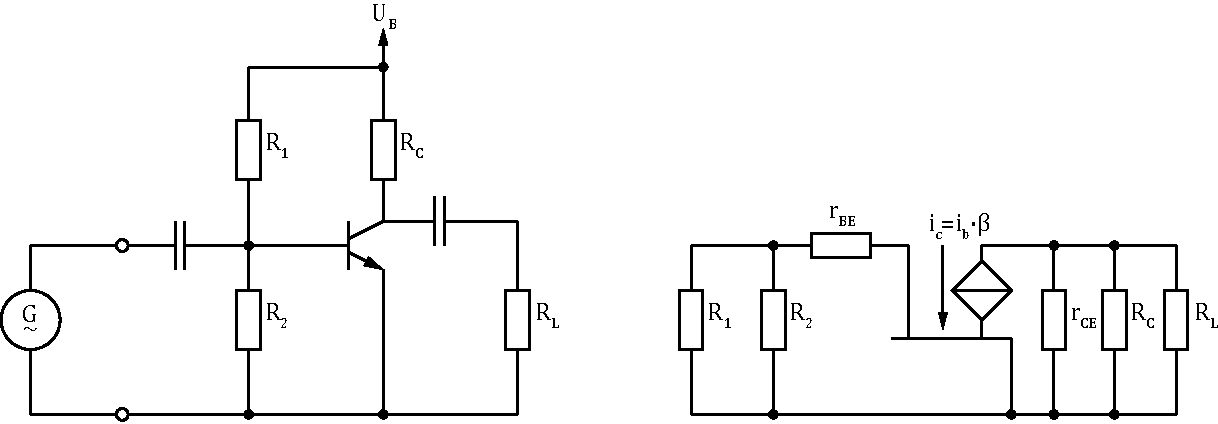
\includegraphics[width = \linewidth]{trans_emitter.pdf}
	\caption{Emitterschaltung mit Kleinsignalersatzschaltbild}
	\label{trans:emitterschaltung}
\end{figure}
\noindent
Spannungsverstärkung:
\[
	V_u = \frac{u_a}{u_e} = \beta \frac{r_{CE} \parallel R_C \parallel R_L}{r_{BE}}
\]
Eingangswiderstand:
\[
	r_e = r_{BE} \parallel R_1 \parallel R_2
\]
Stromverstärkung:
\[
	V_i = \frac{i_a}{i_e} = \beta \frac{r_{CE} \parallel R_C \parallel R_L}{R_L}
\]
Ausgangswiderstand:
\[
	r_a = r_{CE} \parallel R_C
\]

\subsection{Emitterschaltung mit Stromgegenkopplung}
\begin{figure}[h!]
	\centering
	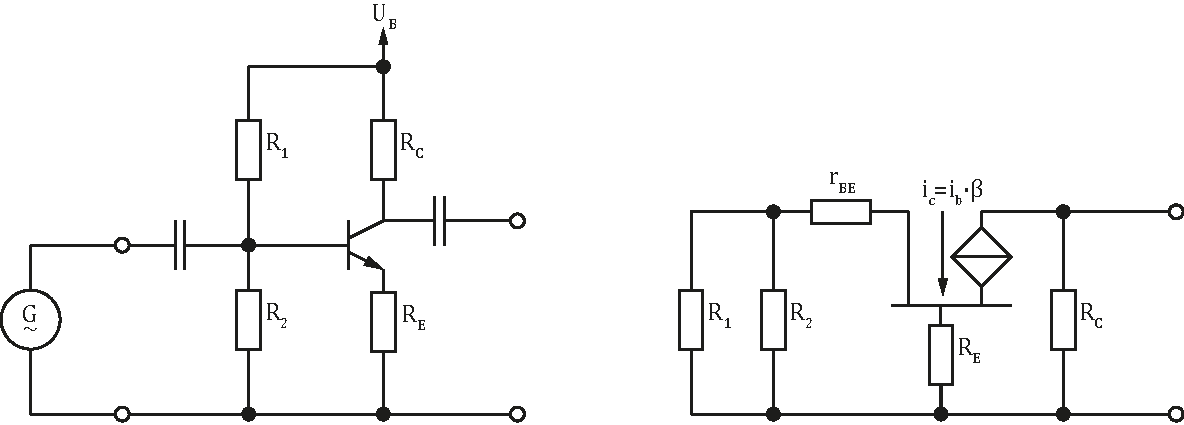
\includegraphics[width = \linewidth]{trans_emitter_stromgegen.pdf}
	\caption{Emitterschaltung mit Stromgegenkopplung und Kleinsignalersatzschaltbild}
	\label{trans:emitterschaltung_sgk}
\end{figure}
\noindent
Kleinsignal Formeln (Näherungen, $r_{CE} = \infty$):
\\\\
Spannungsverstärkung:
\[
	V_U = \frac{u_a}{u_e} = \frac{-\beta \cdot R_C}{r_{BE} + (1 + \beta) \cdot R_E} \approx \frac{-R_C}{R_E}
\]
Eingangswiderstand Transistor:
\[
	r_{eTr} \approx r_{BE} + (\beta + 1) \cdot R_E
\]
Gesammt Eingangswiderstand:
\[
	r_e \approx r_{eTr} \parallel R_1 \parallel R_2
\]
Ausgangswiderstand:
\[
	r_a \approx R_C
\]

\subsection{Emitterschaltung mit Transistorkapazitäten}
\[
	f_{go} = \frac{1}{2\pi \cdot R_q \parallel R_{eTR} \cdot C_{inT}}
\]
\[
	C_{inT} = C_{CB} \cdot (1-V_{ue}) + C_{BE} \cdot (1-V_{uc})
\]
\begin{tabular}{@{}ll}
  $V_{ue}$:	    & Verstärkung der Emitterschaltung ($\frac{U_{C}}{U_{B}}$) \\
  $V_{uc}$:	    & Verstärkung der Kollektorschaltung ($\frac{U_{E}}{U_{B}}$) \\
\end{tabular}

\subsection{Kollektorschaltung}
\begin{figure}[h!]
	\centering
	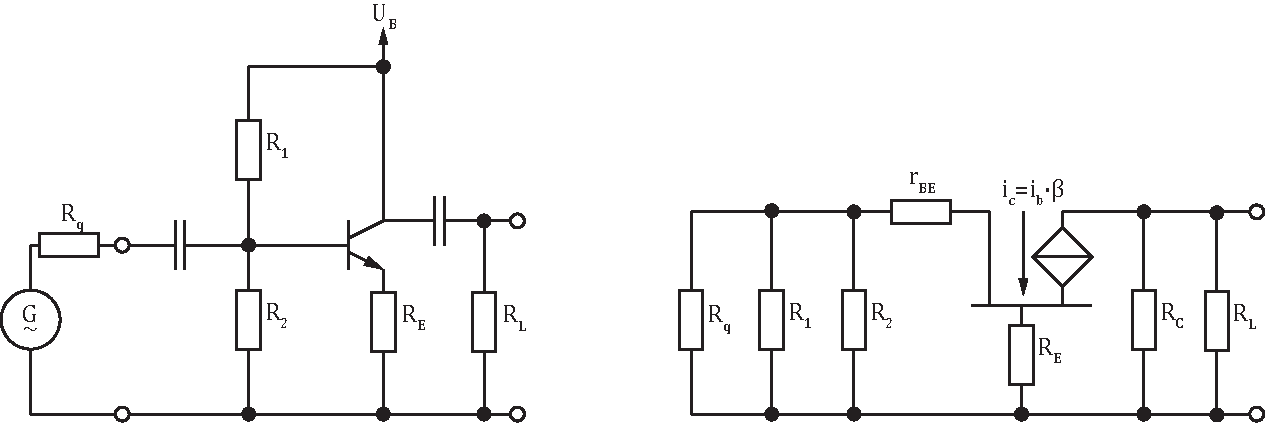
\includegraphics[width = \linewidth]{trans_kollektor.pdf}
	\caption{Kollektorschaltung mit Kleinsignalersatzschaltbild}
	\label{trans:kollektroschaltung}
\end{figure}
\noindent
Verstärkung:
\[
	V_U = \frac{u_a}{u_e} = \frac{1}{1 + \frac{r_{BE}}{(\beta + 1) \cdot R_E \parallel R_L}}
\]
Eingangswiderstand:
\[
	r_e = R_1 \parallel R_2 \parallel (r_{BE} + (\beta+1) \cdot R_E \parallel R_L)
\]
Ausgangswiderstand:
\[
	r_a = R_E \parallel \frac{R_1 \parallel R_2 \parallel R_q + r_{BE}}{\beta + 1}
\]

\subsection{Dalingtonschaltung}
\begin{figure}[h!]
	\centering
	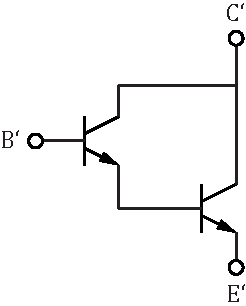
\includegraphics[scale = 0.6]{darlington.pdf}
	\caption{Darlingtonschaltung}
	\label{trans:darlington}
\end{figure}
\noindent
Ersatzkennwerte:
\[ \beta' = \beta_1 \cdot \beta_2 \]
\[ r_{BE}' = 2r_{BE1} \]
\[ r_{CE}' = \frac{2}{3} r_{CE2} \]

\subsection{Komplementär Darlington-Schaltung}
\begin{figure}[h!]
	\centering
	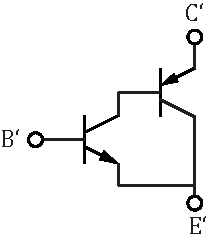
\includegraphics[scale = 0.6]{darlington_komp.pdf}
	\caption{Komplementär Darlington-Schaltung}
	\label{trans:darlington_komp}
\end{figure}
\noindent
Ersatzkennwerte:
\[ \beta' = \beta_1 \cdot \beta_2 \]
\[ r_{BE}' = r_{BE1} \]
\[ r_{CE}' = \frac{1}{2} r_{CE2} \]	        % DC_Grosssignalverhalten

% Unipolartransistor
% coding:utf-8

%FOSAET, a LaTeX-Code for a electrical summary of basic electronics
%Copyright (C) 2013, Daniel Winz, Ervin Mazlagic, Mario Felder

%This program is free software; you can redistribute it and/or
%modify it under the terms of the GNU General Public License
%as published by the Free Software Foundation; either version 2
%of the License, or (at your option) any later version.

%This program is distributed in the hope that it will be useful,
%but WITHOUT ANY WARRANTY; without even the implied warranty of
%MERCHANTABILITY or FITNESS FOR A PARTICULAR PURPOSE.  See the
%GNU General Public License for more details.
%----------------------------------------

\newpage
\section{Feldeffektransistor}

\subsection{Transferkennlinie}
Steilheit:
\[ g_{fs} = \frac{\Delta I_{D}}{\Delta U_{GS}} \]
\[ g_{fs} = k \cdot (U_{GS} - U_t) \]
\[ g_{fs} = \frac{2 \cdot I_D}{U_{GS} - U_t} \]
\begin{tabular}{@{}ll}
  $U_t$:        & Schwellsapnnung, threshold voltage\\
  $k$:	    	& Steilheitskoeffizient oder Transconductance Parameter \\
\end{tabular}

\subsection{Ausgangskennlinie}
\[ r_{DS} = \frac{\Delta U_{DS}}{\Delta I_D}\]

\subsection{Strom- Spannungsbeziehungen}
im Anlaufgebiet, d.h. $u_{GS} \geq U_t$ und $0 < u{DS} < u{GS} - U_t$
\[ i_D = k \cdot \left( (u_{GS} - U_t) \cdot u_{DS} - \frac{1}{2} {u_{DS}}^2 \right) \]
\\
im Sättigungsgebiet, d.h. $u_{GS} > U_t$ und $u_{DS} \geq u_{GS} - U_t$
\[ i_D = \frac{k}{2} (u_{GS} - U_t)^2 \]\\
\begin{tabular}{@{}ll}
  $U_t$:        & Schwellsapnnung, threshold voltage\\
  $k$:	    	& Steilheitskoeffizient oder Transconductance Parameter \\
\end{tabular}
% coding:utf-8

%FOSAET, a LaTeX-Code for a electrical summary of basic electronics
%Copyright (C) 2013, Daniel Winz, Ervin Mazlagic, Mario Felder

%This program is free software; you can redistribute it and/or
%modify it under the terms of the GNU General Public License
%as published by the Free Software Foundation; either version 2
%of the License, or (at your option) any later version.

%This program is distributed in the hope that it will be useful,
%but WITHOUT ANY WARRANTY; without even the implied warranty of
%MERCHANTABILITY or FITNESS FOR A PARTICULAR PURPOSE.  See the
%GNU General Public License for more details.
%----------------------------------------

\subsection{Source Schaltung}
\begin{figure}[h!]
	\centering
	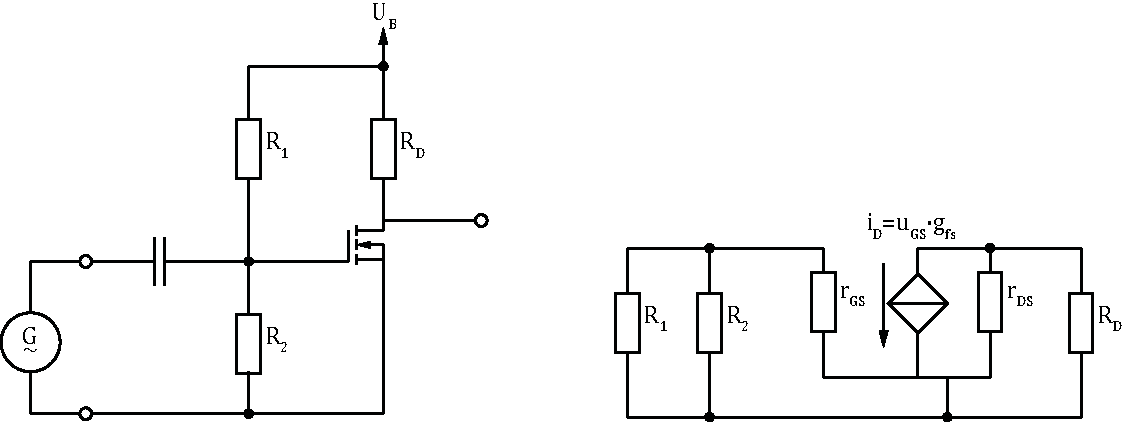
\includegraphics[width = \linewidth]{fet_source.pdf}
	\caption{Source Schaltung und Kleinsignalersatzschaltung}
	\label{fet:sourceschaltung}
\end{figure}
\noindent
Arbeitspunkteinstellung:
\[ U_{AP} = U_B - \frac{U_B - u_{DSmin}}{2} \]
\begin{tabular}{@{}ll}
  $U_B$:        & Quellenspannung
\end{tabular}
\\\\
Spannungsverstärkung:
\[ V_u = -g_{fs} \cdot \frac{R_D \cdot r_{DS}}{R_D + r_{DS}} \]
Ausgangswiderstand:
\[ r_a = \frac{R_D \cdot r_{DS}}{R_D + r_{DS}} \]
Eingangswiderstand:
\[ r_e = \frac{r_{GS} \cdot R_G'}{r_{GS} + R_G'}\]
\[ R_G' = R_1 \parallel R_2 \]
% coding:utf-8

%FOSAET, a LaTeX-Code for a electrical summary of basic electronics
%Copyright (C) 2013, Daniel Winz, Ervin Mazlagic, Mario Felder

%This program is free software; you can redistribute it and/or
%modify it under the terms of the GNU General Public License
%as published by the Free Software Foundation; either version 2
%of the License, or (at your option) any later version.

%This program is distributed in the hope that it will be useful,
%but WITHOUT ANY WARRANTY; without even the implied warranty of
%MERCHANTABILITY or FITNESS FOR A PARTICULAR PURPOSE.  See the
%GNU General Public License for more details.
%----------------------------------------

\subsection{Source Schaltung mit Spannungsgegenkopplung}
\begin{figure}[h!]
	\centering
	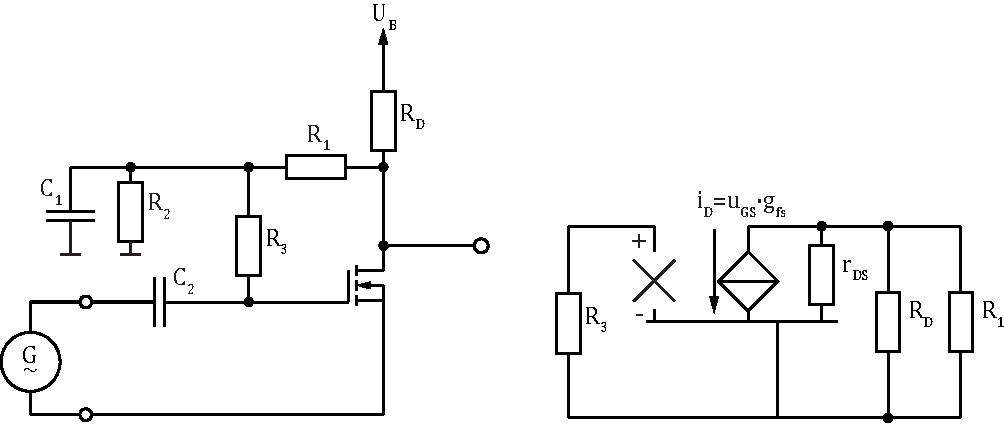
\includegraphics[width = \linewidth]{fet_source_u.pdf}
	\caption{Source Schaltung mit Spannungsgegenkopplung und Kleinsignalersatzschaltung}
	\label{fet:sourceschaltung_u}
\end{figure}
\noindent
\paragraph{Dimensionierung:}
\begin{itemize}
	\item Wahl von $I_D$ aufgrund des nötigen Ausgangswiderstandes $\rightarrow R_D$
	\item Wahl von $R_3$ im Bereich von $100k\Omega$ bis $10M\Omega$
	\item $R_1 \approx 100\cdot R_D$
	\item $R_2 = R_1 \cdot \frac{U_{GS}}{(U_a-U_{GS})}$
	\item Untere Grenfrequenz: $f_{gu} = \frac{1}{2\pi \cdot R_3 \cdot C_2}$
	\item Wahl von $C_1$ dass $C_1 \cdot R_1 \parallel R_2 \gg C_2 \cdot R_3$
\end{itemize}
% coding:utf-8

%FOSAET, a LaTeX-Code for a electrical summary of basic electronics
%Copyright (C) 2013, Daniel Winz, Ervin Mazlagic, Mario Felder

%This program is free software; you can redistribute it and/or
%modify it under the terms of the GNU General Public License
%as published by the Free Software Foundation; either version 2
%of the License, or (at your option) any later version.

%This program is distributed in the hope that it will be useful,
%but WITHOUT ANY WARRANTY; without even the implied warranty of
%MERCHANTABILITY or FITNESS FOR A PARTICULAR PURPOSE.  See the
%GNU General Public License for more details.
%----------------------------------------

\subsection{Source Schaltung mit Stromgegenkopplung}
\begin{figure}[h!]
	\centering
	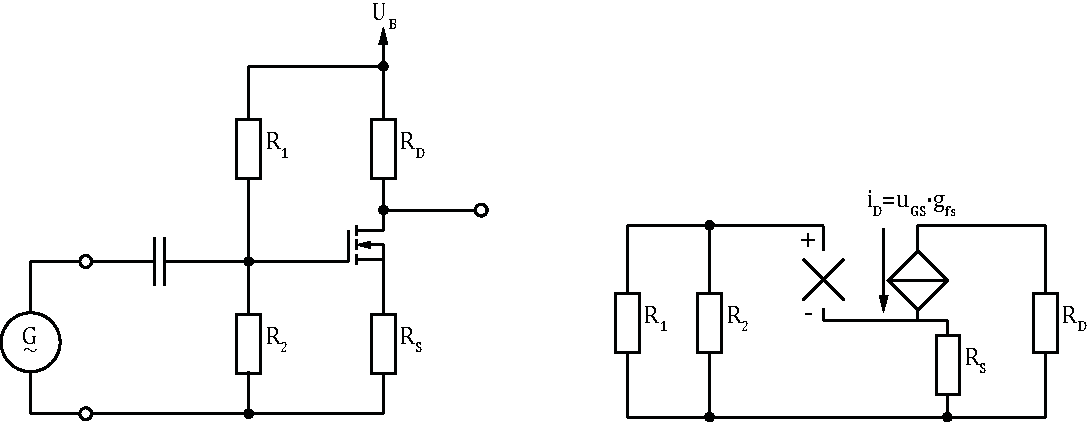
\includegraphics[width = \linewidth]{fet_source_i.pdf}
	\caption{Source Schaltung mit Stromgegenkopplung und Kleinsignalersatzschaltung}
	\label{fet:sourceschaltung_i}
\end{figure}
\noindent
\paragraph{Dimensionierung:}
\begin{itemize}
	\item Wahl von $I_D$ aufgrund des nötigen Ausgangswiderstandes $\rightarrow R_D$
	\item Wahl von $R_S$ für ein $U_{RS}$ von ca. $1V$
	\item Wahl von $R_2$ im Bereich von $100k\Omega$ bis $10M\Omega$
	\item $R_1 = R_2 \cdot \frac{U_B - U_{GS} - U_{RS}}{(U_{GS}+U_{RS})}$
	\item Untere Grenfrequenz: $f_{gu} = \frac{1}{2\pi \cdot C_2 \cdot R_1 \parallel R_2}$
\end{itemize}
\noindent\\
Spannungsverstärkung:
\[
	V_u = \frac{U_a}{U_e} = \frac{-g_{fs} \cdot R_D}{R_S \cdot g_{fs} + 1}
\]
Eingangswiderstand:
\[
	r_e = R_1 \parallel R_2
\]
Ausgangswiderstand:
\[
	r_a = R_D
\]
(Annahme: $r_{DS} \gg R_D$)
% coding:utf-8

%FOSAET, a LaTeX-Code for a electrical summary of basic electronics
%Copyright (C) 2013, Daniel Winz, Ervin Mazlagic, Mario Felder

%This program is free software; you can redistribute it and/or
%modify it under the terms of the GNU General Public License
%as published by the Free Software Foundation; either version 2
%of the License, or (at your option) any later version.

%This program is distributed in the hope that it will be useful,
%but WITHOUT ANY WARRANTY; without even the implied warranty of
%MERCHANTABILITY or FITNESS FOR A PARTICULAR PURPOSE.  See the
%GNU General Public License for more details.
%----------------------------------------

\subsection{Drain Schaltung}
\begin{figure}[h!]
	\centering
	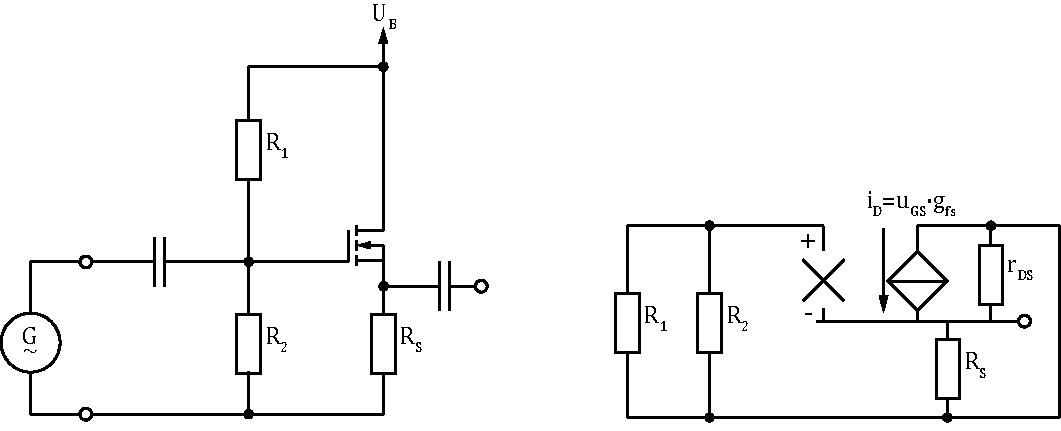
\includegraphics[width = \linewidth]{fet_drain.pdf}
	\caption{Drain Schaltung und Kleinsignalersatzschaltung}
	\label{fet:drainschaltung}
\end{figure}
\noindent
Spannungsverstärkung:
\[
	V_u = \frac{r_{DS} \parallel R_S}{r_{DS} \parallel R_S + \frac{1}{g_{fs}}} \approx 1
\]
Ausganswiderstand:
\[
	r_a = \frac{1}{g_{fs}} \parallel r_{DS} \parallel R_S
\]
Eingagnswiderstand:
\[
	r_e = (r_{GS} \cdot R_S \cdot g_{fs} + R_S + r_{GS}) \parallel R_1 \parallel R_2
\]
für $r_{GS} = \infty$:
\[
	r_e = R_1 \parallel R_2
\]

% Operationsverstärker
\newpage
\input{op}              % Operationsverstärker
% coding:utf-8

%FOSAET, a LaTeX-Code for a electrical summary of basic electronics
%Copyright (C) 2013, Daniel Winz, Ervin Mazlagic

%This program is free software; you can redistribute it and/or
%modify it under the terms of the GNU General Public License
%as published by the Free Software Foundation; either version 2
%of the License, or (at your option) any later version.

%This program is distributed in the hope that it will be useful,
%but WITHOUT ANY WARRANTY; without even the implied warranty of
%MERCHANTABILITY or FITNESS FOR A PARTICULAR PURPOSE.  See the
%GNU General Public License for more details.
%----------------------------------------


\subsection{Frequenzgang - Realer OP}
\[ V_{U_O} \cdot f_{go} = 1 \cdot f_T \]
Wird mit dem Operationsverstärker ein Filter mit Güte realisiert, so 
muss die Güte des Filters berücksichtigt werden. 
\[ V_{U_O} \cdot f_{go} \cdot Q = 1 \cdot f_T \]
\begin{tabular}{@{}ll}
  $V_{U_O}$:    & Openloop Versärkung DC \\
  $f_{go}$:     & Openloop Grenzfrequenz \\   
  $f_T$:        & Transitfrequenz \\
  $Q$:          & Güte \\
\end{tabular}
        % Frequenzgang
\input{op_ausgang}      % Verhalten am Ausgang
\newpage
\input{op_ufolg}        % Spannungsfolger, Impedanzwandler
% coding:utf-8

%FOSAET, a LaTeX-Code for a electrical summary of basic electronics
%Copyright (C) 2013, Daniel Winz, Ervin Mazlagic

%This program is free software; you can redistribute it and/or
%modify it under the terms of the GNU General Public License
%as published by the Free Software Foundation; either version 2
%of the License, or (at your option) any later version.

%This program is distributed in the hope that it will be useful,
%but WITHOUT ANY WARRANTY; without even the implied warranty of
%MERCHANTABILITY or FITNESS FOR A PARTICULAR PURPOSE.  See the
%GNU General Public License for more details.
%----------------------------------------

\subsection{Nichtinvertierender Verstärker}
\begin{figure}[h!]
	\centering
	\includegraphics[scale=\schscale]{../fig/op_ninv.pdf}
	\caption{Nichtinvertierender Verstärker}
	\label{sch:op-ninv}
\end{figure}
\[ V_u = \frac{R_1}{R_2} + 1 \]
\[ U_a = U_e \cdot \frac{R_1}{R_2} + 1 \]
\[ R_e = \infty \]
\[ R_a = 0 \]         % Nichtinvertierender Verstärker
% coding:utf-8

%FOSAET, a LaTeX-Code for a electrical summary of basic electronics
%Copyright (C) 2013, Daniel Winz, Ervin Mazlagic

%This program is free software; you can redistribute it and/or
%modify it under the terms of the GNU General Public License
%as published by the Free Software Foundation; either version 2
%of the License, or (at your option) any later version.

%This program is distributed in the hope that it will be useful,
%but WITHOUT ANY WARRANTY; without even the implied warranty of
%MERCHANTABILITY or FITNESS FOR A PARTICULAR PURPOSE.  See the
%GNU General Public License for more details.
%----------------------------------------

\subsection{Invertierender Verstärker}
\begin{figure}[h!]
	\centering
	\includegraphics[scale=\schscale]{../fig/op_inv.pdf}
	\caption{Invertierender Verstärker}
	\label{sch:op-inv}
\end{figure}
\[ V_u = - \frac{R_2}{R_1} \]
\[ U_a = - U_e \cdot \frac{R_2}{R_1} \]
\[ R_e = R_1 \qquad R_a = 0 \]          % Invertierender Verstärker
% coding:utf-8

%FOSAET, a LaTeX-Code for a electrical summary of basic electronics
%Copyright (C) 2013, Daniel Winz, Ervin Mazlagic

%This program is free software; you can redistribute it and/or
%modify it under the terms of the GNU General Public License
%as published by the Free Software Foundation; either version 2
%of the License, or (at your option) any later version.

%This program is distributed in the hope that it will be useful,
%but WITHOUT ANY WARRANTY; without even the implied warranty of
%MERCHANTABILITY or FITNESS FOR A PARTICULAR PURPOSE.  See the
%GNU General Public License for more details.
%----------------------------------------

\subsection{Addierer}
\begin{figure}[h!]
	\centering
	\includegraphics[scale=\schscale]{../fig/op_add.pdf}
	\caption{Addierer}
	\label{sch:op-add}
\end{figure}
\[ U_a = - R_2 \cdot \left( \frac{U_{e1}}{R_{11}} + \frac{U_{e2}}{R_{12}} 
+ \frac{U_{e3}}{R_{13}} \right) \]
\[ R_{e1} = R_{11} \qquad R_{e2} = R_{12} \qquad R_{e3} = R_{13} \]
\[ R_a = 0 \]
          % Addierer
% coding:utf-8

%FOSAET, a LaTeX-Code for a electrical summary of basic electronics
%Copyright (C) 2013, Daniel Winz, Ervin Mazlagic

%This program is free software; you can redistribute it and/or
%modify it under the terms of the GNU General Public License
%as published by the Free Software Foundation; either version 2
%of the License, or (at your option) any later version.

%This program is distributed in the hope that it will be useful,
%but WITHOUT ANY WARRANTY; without even the implied warranty of
%MERCHANTABILITY or FITNESS FOR A PARTICULAR PURPOSE.  See the
%GNU General Public License for more details.
%----------------------------------------

\subsection{Subtrahierer / Differenzverstärker}
\begin{figure}[h!]
	\centering
	\includegraphics[scale=\schscale]{op_sub.pdf}
	\caption{Subtrahierer / Differenzverstärker}
	\label{sch:op-sub}
\end{figure}
\[ U_a = \frac{(R_1 + R_2) \cdot R_4}{(R_3 + R_4) \cdot R_1} \cdot U_{e+} 
- \frac{R_2}{R_1} \cdot U_{e-} \]
Wenn $R_1 = R_3$ und $R_2 = R_4$: 
\[ U_a = \frac{R_2}{R_1} \cdot (U_{e+} - U_{e-}) \]
Wenn $R_1 = R_2 = R_3 = R_4$: 
\[ U_a = U_{e+} - U_{e-} \]
\[ R_{e+} = R_3 + R_4 \]
\[ R_{e-} = R_1 \]
\[ R_a = 0 \]          % Subtrahierer
\newpage
% coding:utf-8

%FOSAET, a LaTeX-Code for a electrical summary of basic electronics
%Copyright (C) 2013, Daniel Winz, Ervin Mazlagic

%This program is free software; you can redistribute it and/or
%modify it under the terms of the GNU General Public License
%as published by the Free Software Foundation; either version 2
%of the License, or (at your option) any later version.

%This program is distributed in the hope that it will be useful,
%but WITHOUT ANY WARRANTY; without even the implied warranty of
%MERCHANTABILITY or FITNESS FOR A PARTICULAR PURPOSE.  See the
%GNU General Public License for more details.
%----------------------------------------

\subsection{Differenzierer}
\begin{figure}[h!]
	\centering
	\includegraphics[scale=\schscale]{../fig/op_diff.pdf}
	\caption{Differenzierer}
	\label{sch:op-diff}
\end{figure}
\[ U_a = - R \cdot C \cdot \frac{d U_e(t)}{dt} \]
\[ X_e = \frac{1}{j \cdot \omega \cdot f \cdot C} \]
\[ R_a = 0 \]         % Differenzierer
% coding:utf-8

%FOSAET, a LaTeX-Code for a electrical summary of basic electronics
%Copyright (C) 2013, Daniel Winz, Ervin Mazlagic

%This program is free software; you can redistribute it and/or
%modify it under the terms of the GNU General Public License
%as published by the Free Software Foundation; either version 2
%of the License, or (at your option) any later version.

%This program is distributed in the hope that it will be useful,
%but WITHOUT ANY WARRANTY; without even the implied warranty of
%MERCHANTABILITY or FITNESS FOR A PARTICULAR PURPOSE.  See the
%GNU General Public License for more details.
%----------------------------------------

\subsection{Integrierer}
\begin{figure}[h!]
	\centering
	\includegraphics[scale=\schscale]{../fig/op_int.pdf}
	\caption{Integrierer}
	\label{sch:op-int}
\end{figure}
\[ U_a = - \frac{\int_{0}^{t} U_e(t) dt}{R \cdot C} + U_a(0) \]
\[ R_e = R \]
\[ R_a = 0 \]          % Integrierer
\newpage
\input{op_isource}      % Stromquelle
\input{op_iu}           % Strom-Spannungswandler
\input{op_tp_o1_inv}    % Invertierender aktiver Tiefpass 1. Ordnung
% coding:utf-8

%FOSAET, a LaTeX-Code for a electrical summary of basic electronics
%Copyright (C) 2013, Daniel Winz, Ervin Mazlagic

%This program is free software; you can redistribute it and/or
%modify it under the terms of the GNU General Public License
%as published by the Free Software Foundation; either version 2
%of the License, or (at your option) any later version.

%This program is distributed in the hope that it will be useful,
%but WITHOUT ANY WARRANTY; without even the implied warranty of
%MERCHANTABILITY or FITNESS FOR A PARTICULAR PURPOSE.  See the
%GNU General Public License for more details.
%----------------------------------------

\subsection{Invertierender aktiver Hochpass erster Ordnung}
\begin{figure}[h!]
	\centering
	\includegraphics[scale=\schscale]{op_hp_o1_inv.pdf}
	\caption{Invertierender aktiver Hochpass erster Ordnung}
	\label{sch:op-hp-o1-inv}
\end{figure}
\[ H_0 = - \frac{R_2}{R_1} \]
\[ \omega_0 = \frac{1}{R_1 \cdot C} \]
\[ f_0 = \frac{1}{2 \pi \cdot R_1 \cdot C} \]    % Invertierender aktiver Hochpass 1. Ordnung
\newpage
% coding:utf-8

%FOSAET, a LaTeX-Code for a electrical summary of basic electronics
%Copyright (C) 2013, Daniel Winz, Ervin Mazlagic

%This program is free software; you can redistribute it and/or
%modify it under the terms of the GNU General Public License
%as published by the Free Software Foundation; either version 2
%of the License, or (at your option) any later version.

%This program is distributed in the hope that it will be useful,
%but WITHOUT ANY WARRANTY; without even the implied warranty of
%MERCHANTABILITY or FITNESS FOR A PARTICULAR PURPOSE.  See the
%GNU General Public License for more details.
%----------------------------------------

\subsection{Aktiver Tiefpass 2. Ordnung}
\label{filt:o2-tp}
\begin{figure}[h!]
	\centering
	\includegraphics[scale=\schscale]{op_tp_o2.pdf}
	\caption{Aktiver Tiefpass 2. Ordnung}
	\label{sch:op-tp-o2}
\end{figure}
\[ \frac{-H \cdot {\omega_0}^2}
{s^2 + \alpha \cdot \omega_0 \cdot s + {\omega_0}^2} \]
\[ \frac{V_{out}}{V_{in}} 
= \frac{-H \cdot \frac{1}{R_3 \cdot R_4 \cdot C_2 \cdot C_5}}
{s^2 + s \cdot \frac{1}{C_2} 
\left(\frac{1}{R_1} + \frac{1}{R_3} + \frac{1}{R_4}\right) 
+ \frac{1}{R_3 \cdot R_4 \cdot C_2 \cdot C_5}} \]
\[ \alpha = \frac{1}{Q} \]

\subsubsection{Dimensionierung}
\[ C_5 \text{ wählen} \]
\[ k = 2 \pi \cdot f_0 \cdot C_5 \]
\[ C_2 = \frac{4}{\alpha^2} (H + 1) \cdot C_5 
= 4 \cdot Q^2 (H + 1) \cdot C_5 \]
\[ R_1 = \frac{\alpha}{2 \cdot H \cdot k} 
= \frac{1}{2 \cdot Q \cdot H \cdot k} \]
\[ R_3 = \frac{\alpha}{2 \cdot (H + 1) \cdot k} 
= \frac{1}{2 \cdot Q \cdot (H + 1) \cdot k} \]
\[ R_4 = \frac{\alpha}{2 \cdot k} = \frac{1}{2 \cdot Q \cdot k} \]
        % Aktiver Tiefpass 2. Ordnung
\newpage
% coding:utf-8

%FOSAET, a LaTeX-Code for a electrical summary of basic electronics
%Copyright (C) 2013, Daniel Winz, Ervin Mazlagic

%This program is free software; you can redistribute it and/or
%modify it under the terms of the GNU General Public License
%as published by the Free Software Foundation; either version 2
%of the License, or (at your option) any later version.

%This program is distributed in the hope that it will be useful,
%but WITHOUT ANY WARRANTY; without even the implied warranty of
%MERCHANTABILITY or FITNESS FOR A PARTICULAR PURPOSE.  See the
%GNU General Public License for more details.
%----------------------------------------

\subsection{Aktiver Hochpass 2. Ordnung}
\label{filt:o2-hp}
\begin{figure}[h!]
	\centering
	\includegraphics[scale=\schscale]{../fig/op_hp_o2.pdf}
	\caption{Aktiver Hochpass 2. Ordnung}
	\label{sch:op-hp-o2}
\end{figure}
\[ \frac{-H \cdot s^2}{s^2 + \alpha \cdot \omega_0 \cdot s + {\omega_0}^2} \]
\[ \frac{V_{out}}{V_{in}} = \frac{- s^2 \cdot \frac{C_1}{C_4}}
{s^2 + s \cdot \frac{C_1 + C_3 + C_4}{C_3 \cdot C_4 \cdot R_5} 
+ \frac{1}{R_2 \cdot R_5 \cdot C_3 \cdot C_4}} \]
\[ \alpha = \frac{1}{Q} \]
\subsubsection{Dimensionierung}
\[ C_1 \text{ wählen} \]
\[ k = 2 \cdot \pi \cdot f_0 \cdot C_1 \]
\[ C_3 = C_1 \]
\[ C_4 = \frac{C_1}{H} \]
\[ R_2 = \frac{\alpha}{k \cdot \left(2 + \frac{1}{H}\right)} 
= \frac{1}{Q \cdot k \cdot \left(2 + \frac{1}{H}\right)} \]
\[ R_5 = \frac{H \cdot \left(2 + \frac{1}{H}\right)}{\alpha \cdot k} 
= \frac{Q \cdot H \cdot \left(2 + \frac{1}{H}\right)}{k} \]
        % Aktiver Hochpass 2. Ordnung
\newpage
% coding:utf-8

%FOSAET, a LaTeX-Code for a electrical summary of basic electronics
%Copyright (C) 2013, Daniel Winz, Ervin Mazlagic

%This program is free software; you can redistribute it and/or
%modify it under the terms of the GNU General Public License
%as published by the Free Software Foundation; either version 2
%of the License, or (at your option) any later version.

%This program is distributed in the hope that it will be useful,
%but WITHOUT ANY WARRANTY; without even the implied warranty of
%MERCHANTABILITY or FITNESS FOR A PARTICULAR PURPOSE.  See the
%GNU General Public License for more details.
%----------------------------------------

\subsection{Aktiver Bandpass 2. Ordnung}
\begin{figure}[h!]
	\centering
	\includegraphics[scale=\schscale]{op_bp_o2.pdf}
	\caption{IAktiver Bandpass 2. Ordnung}
	\label{sch:op-bp-o2}
\end{figure}
\[ \frac{- H \cdot \omega_0 \cdot s}
{s^2 + \alpha \cdot \omega_0 \cdot s  + {\omega_0}^2} \]
\[ \frac{V_{out}}{V_{in}} = \frac{- s \cdot \frac{1}{R_1 \cdot C_4}}
{s^2 + s \cdot \frac{C_3 + C_4}{C_3 \cdot C_4 \cdot R_5} + 
\frac{1}{R_5 \cdot C_3 \cdot C_4} \cdot 
\left(\frac{1}{R_1} + \frac{1}{R_2}\right)} \]
\[  \alpha = \frac{1}{Q}\]
\subsubsection{Dimensionierung}
\[ C_3 \text{ wählen} \]
\[ k = 2 \pi \cdot f_0 \cdot C_3 \]
\[ C_4 = C_3 \]
\[ R_1 = \frac{1}{H \cdot k} \]
\[ R_2 = \frac{1}{(2 \cdot Q - H) \cdot k} \]
\[ R_5 = \frac{2 \cdot Q}{k} \]        % Aktiver Bandpass 2. Ordnung
% coding:utf-8

%FOSAET, a LaTeX-Code for a electrical summary of basic electronics
%Copyright (C) 2013, Daniel Winz, Ervin Mazlagic

%This program is free software; you can redistribute it and/or
%modify it under the terms of the GNU General Public License
%as published by the Free Software Foundation; either version 2
%of the License, or (at your option) any later version.

%This program is distributed in the hope that it will be useful,
%but WITHOUT ANY WARRANTY; without even the implied warranty of
%MERCHANTABILITY or FITNESS FOR A PARTICULAR PURPOSE.  See the
%GNU General Public License for more details.
%----------------------------------------

\section{Filter höherer Ordnung}
Filter höherer Ordunung können aus Filtern erster und zweiter Ordnung 
zusammengesetzt werden. Dabei können die einzelnen Filter parallel oder in 
Kaskadenform kombiniert werden. Die Kaskadenform wird dabei weitaus häufiger 
verwendet. 

\subsection{Bestimmen der Ordnung}
Butterworth Filter
\[ N \geq \frac{\log_{10}\left(\dfrac{\lambda}{\epsilon}\right)}
{\log_{10}\left(\dfrac{f_s}{f_g}\right)} 
= \frac{\log_{10}\left(\sqrt{\dfrac{10^{(0.1 \cdot A_{min_{dB}})} - 1}
{10^{(0.1 \cdot A_{max_{dB}})} - 1}}\right)}
{\log_{10}\left(\dfrac{f_s}{f_g}\right)} 
= \frac{\log_{10}\left(\sqrt{\dfrac{\frac{1}{{A_{min}}^2} - 1}
{\frac{1}{{A_{max}}^2} - 1}}\right)}
{\log_{10}\left(\dfrac{f_s}{f_g}\right)} \]
Tschebyscheff Filter
\[ N \geq \frac{\arccosh\left(\dfrac{\lambda}{\epsilon}\right)}
{\arccosh\left(\dfrac{f_s}{f_g}\right)} 
= \frac{\arccosh\left(\sqrt{\dfrac{10^{(0.1 \cdot A_{min_{dB}})} - 1}
{10^{(0.1 \cdot A_{max_{dB}})} - 1}}\right)}
{\arccosh\left(\dfrac{f_s}{f_g}\right)} 
= \frac{\arccosh\left(\sqrt{\dfrac{\frac{1}{{A_{min}}^2} - 1}
{\frac{1}{{A_{max}}^2} - 1}}\right)}
{\arccosh\left(\dfrac{f_s}{f_g}\right)} \]

      % Filter höherer Ordnung

% Kühlung
\newpage
% coding:utf-8

%FOSAET, a LaTeX-Code for a electrical summary of basic electronics
%Copyright (C) 2013, Daniel Winz, Ervin Mazlagic

%This program is free software; you can redistribute it and/or
%modify it under the terms of the GNU General Public License
%as published by the Free Software Foundation; either version 2
%of the License, or (at your option) any later version.

%This program is distributed in the hope that it will be useful,
%but WITHOUT ANY WARRANTY; without even the implied warranty of
%MERCHANTABILITY or FITNESS FOR A PARTICULAR PURPOSE.  See the
%GNU General Public License for more details.
%----------------------------------------

\section{Thermisches Ersatzschaltbild}
\begin{figure}[h!]
  \centering
  \begin{circuitikz}[scale=1]\draw
%     (0,0) to[short, o-] (0,0)
%     (0,0) to[short, -o] (0,0)
    (0,6) to[R=$R_{th_{JC}}$, o-o] (0,4)
    (0,4) to[R=$R_{th_{CH}}$, o-o] (0,2)
    (0,2) to[R=$R_{th_{HA}}$, o-o] (0,0)
    (0.4,6) node {J}
    (0.4,4) node {C}
    (0.4,2) node {H}
    (0.4,0) node {A}
    ;
  \end{circuitikz}
  \caption{Thermisches Ersatzschaltbild}
\end{figure}
Äquivalent zu Ohmschem Gesetz: 
\[ \Delta\vartheta = R_{th} \cdot P_v \]
\[ R_{th} = \frac{\ell}{\lambda \cdot A} \]
\begin{tabular}{@{}ll}
  $J$: & Junction $\rightarrow$ Sperrschicht \\
  $C$: & Case $\rightarrow$ Gehäuse \\
  $H$: & Heatsink $\rightarrow$ Kühlkörper \\
  $A$: & Ambient $\rightarrow$ Umgebung (Achtung! Meist innerhalb Gerät) \\
  $\lambda$: & Thermische Leitfähigkeit
\end{tabular}
         % Thermisches Ersatzschaltbild
